%% Submissions for peer-review must enable line-numbering
%% using the lineno option in the \documentclass command.
%%
%% Preprints and camera-ready submissions do not need
%% line numbers, and should have this option removed.
%%
%% Please note that the line numbering option requires
%% version 1.1 or newer of the wlpeerj.cls file.

\documentclass[fleqn,10pt,lineno]{wlpeerj} % for journal submissions
% \documentclass[fleqn,10pt]{wlpeerj} % for preprint submissions

\newcommand{\cheng}[1]{\textcolor{green}{\textbf{Cheng: }{\footnotesize #1}}}
\newcommand{\alasdair}[1]{\textcolor{blue}{\textbf{Alasdair: }{\footnotesize #1}}}

\usepackage{bm} % bold math symbols
\usepackage{hyperref} % create hyperlinks
\usepackage[labelfont=bf]{caption} % figure captions
\usepackage{algorithm} 
\usepackage{algpseudocode} % display algorithms in pseudo-code

\hypersetup{
	colorlinks   = true, % Colours links instead of ugly boxes
	pdfauthor    = {Alasdair Tran and Cheng Soon Ong},
	pdftitle	 = {Combining Active Learning Suggestions},
}

% some convenient symbols
\DeclareMathAlphabet{\mathpzc}{OT1}{pzc}{m}{it}
\DeclareMathOperator{\Beta}{Beta}
\DeclareMathOperator{\Bin}{Bin}
\DeclareMathOperator{\tr}{tr}
\newcommand{\A}{\mathpzc{A}}
\newcommand{\B}{\mathcal{B}}
\newcommand{\X}{\mathcal{X}}
\newcommand{\Y}{\mathcal{Y}}
\newcommand{\Ecal}{\mathcal{E}}
\newcommand{\Normal}{\mathcal{N}}
\newcommand{\Unlabelled}{\mathcal{U}}
\newcommand{\Labelled}{\mathcal{L}}
\newcommand{\R}{\mathcal{R}}
\newcommand*{\argmin}{\operatornamewithlimits{argmin}\limits}
\newcommand*{\argmax}{\operatornamewithlimits{argmax}\limits}


\title{Combining Active Learning Suggestions}

\author[1]{Alasdair Tran}
\author[2]{Cheng Soon Ong}
\affil[1]{}
\affil[2]{Machine Learning Research Group, Data61, CSIRO, Australia}

\keywords{machine learning, astronomy, active learning, bandit, rank aggregation}

\begin{abstract}
Recent advances in sensors and scientific instruments have led to an increasing use of machine
learning techniques for managing the data deluge. Supervised learning has become a widely used
paradigm in many big data applications. However,  labeled examples are required during the
training phase of supervised machine learning algorithms, and the labeling has become a 
significant bottleneck. This paper explores the use of machine learning algorithms for 
identifying informative examples for labeling, the so-called active learning setting. We 
empirically compare several active learning heuristics on benchmark datasets, and focus on its 
application to photometric classification of the Sloan Digital Sky Survey. By considering each 
active learning heuristic as an expert recommendation of which example to label, we propose to 
combine them using bandit and rank aggregation algorithms. Our results show that combining 
active learning suggestions improves over each individual heuristic (including passive 
learning), and provides a promising practical approach.
\end{abstract}

\begin{document}

\flushbottom
\maketitle
\thispagestyle{empty}

\section*{Introduction}

There are three ideas which are often used to elicit human responses -
active learning, bandits, and experimental designs. These ideas are
similar in spirits



Previous surveys~\cite{baram04, hsu15}.
We are more comprehensive, and consider other types of combination.
There are three ideas which are often used for eliciting human
responses using machine learning predictors. At a high level they are
similar is spirit, but they have different foundations which lead to
different formulations. The ideas are active learning, bandits and
experimental design. Related to this but with literature from a
different field is social choice theory, which looks at
how individual preferences are aggregated.

\subsection*{Active Learning}

Active learning considers the setting where the agent interacts with
its environment to procure a training set, rather than passively
receiving i.i.d. samples from some underlying distribution.

It is often assumed that the environment is infinite (e.g. $R^d$) and
the agent has to choose a location, $x$, to query. The oracle then returns
the label $y$. It is often assumed that there is no noise in the label,
and hence there is no benefit of querying the same point $x$ again. In
many practical applications, the environment is considered to be
finite (but large). This is called the pool-based active learning.

The active learning algorithm is often compared to the passive
learning algorithm.

\subsection*{Bandits}

A bandit problem is a sequential allocation problem defined by a set
of actions. The agent chooses an action at each time step, and the
environment returns a reward. The aim of the agent is to maximise reward.

In basic settings, the set of actions is considered to be
finite. There are three fundamental formalisations of the bandit
problem, depending on the assumed nature of the reward process:
stochastic, adversarial and Markovian. In all three settings the
reward is uncertain, and hence the agent may have to play a particular
action repeatedly.

The agent is compared to a static agent which has played the best
action. This difference in reward is called regret.

\subsection*{Choice: Rank aggregation}

http://plato.stanford.edu/entries/social-choice/

\begin{itemize}
  \item Pairwise majority rule
  \item Borda count
  \item geometric mean http://arxiv.org/abs/1410.4391
\end{itemize}


\subsection*{Experimental Design}

In contrast to active learning, experimental design considers the problem of regression, i.e. where the label $y\in R$ is a real number.

The problem to be solved in experimental design is to choose a set of
trials (say of size N) to gather enough information about the object
of interest. The goal is to maximise the information obtained about
the parameters of the model (of the object).

It is often assumed that the observations at the N trials are
independent. When N is finite this is called exact design, otherwise
it is called approximate or continuous design. The environment is
assumed to be infinite (e.g. $R^d$) and the observations are scalar real variables.

\section*{Problem Formulation}

Suppose we have a classifier $h$ that maps the input space

We shall consider eight active learning suggestions:

\begin{table}[h]
	\caption {Summary of active learning heuristics used in our experiments} \label{tab:heuristics}
	\centering
	\begin{tabular}{lll}
		\toprule
		{Name}  & Notation &  Objective  \\
		\midrule
		Entropy & $r_S(\bm{x}; h)$
			& $\argmax_{x \in \Ecal} \left\{-\sum_{y \in \Y} p(y | \bm{x}; h)
            \log \big[ p(y | \bm{x}; h) \big] \right\}$
			\\[2ex]
		Margin & $r_M(\bm{x}; h)$
			& $\argmin_{x \in \Ecal} \left\{ \max_{y \in \Y} p(y | \bm{x}; h) -
            \max_{z \in \Y \setminus \{y\}} p(z | \bm{x}; h)  \right\}$
			\\[2ex]
		QBB Margin & $r_{QM}(\bm{x}; h)$
			& $\argmin_{x \in \Ecal} \left\{ \max_{y \in \Y} p(y | \bm{x}; \B) -
            \max_{z \in \Y \setminus \{y\}} p(z | \bm{x}; \B)  \right\}$
			\\[2ex]
		QBB KL & $r_{QK}(\bm{x}; h)$
			& $\argmax_{x \in \Ecal} \left\{ \dfrac{1}{B}
               \sum_{b=1}^B D_{\mathrm{KL}}(p_b\|p_\B) \right\}$
			\\
        Confidence & $r_{C}(\bm{x}; h)$
			& $\argmax_{x \in \Ecal} \left\{   \right\}$
			\\
        Weighted Margin &
			&
			\\
		\bottomrule
	\end{tabular}
\end{table}

Reward: improvement in balanced accuracy.

\section*{Combining Suggestions}

We study four bandit algorithms: KL-UCB \cite{cappe13}, OC-UCB \cite{lattimore15}, EXP3++ \cite{seldin14}, and Thompson sampling.


\algblock[Name]{Start}{End}
\algblockdefx[Forall]{Foreach}{Endforeach}%
			[1]{\textbf{for each} #1 \textbf{do}}%
			{\textbf{end for}}

\begin{algorithm}[tbp]
	\caption{Thompson sampling} \index{bandit}
	\label{alg:bandit}
	\begin{algorithmic}[1]
		\Procedure {ThompsonSampling}{$\Unlabelled$, $\Labelled_T$, $h$, $n$, $E$,
			                      $\R$, $\bm{\mu}$, $\bm{\sigma}^2$, $\bm{\tau}^2$}
    		\While {$|\Labelled_T| < n$}
        		\Foreach  {$i \in \{1, 2, ..., |\R|\}$}
        			\State $\nu_i' \leftarrow$ draw a sample from $\Normal(\mu_i, \sigma^2_i)$
        		\Endforeach
        		\State $r_* \leftarrow \argmax_{i} \nu_i'$
        		\State $\Ecal$ $\leftarrow$ random sample of size $E$ from $\Unlabelled$
        		\State $\bm{x}_* \leftarrow \argmax_{\bm{x} \in \Ecal} r_*(\bm{x})$
        		\State $y_* \leftarrow$ ask the expert to label $\bm{x}_*$
        		\State $\Labelled_T \leftarrow \Labelled_T  \cup (\bm{x}_*, y_*)$
        		\State $\Unlabelled \leftarrow \Unlabelled \setminus \bm{x}_*$
        		\State $h(\bm{x}) \leftarrow$ retrain the classifier
        		\State $\delta$ $\leftarrow$ incremental increase in the accuracy
        		\State $\mu_* \leftarrow \dfrac{\mu_* \tau^2_* + \delta \sigma^2_*}{\sigma^2_* + \tau^2_*}$
                \State $\sigma_*^2 \leftarrow \dfrac{\sigma^2_* \tau^2_*}{\sigma^2_* + \tau^2_*}$
    		\EndWhile
		\EndProcedure
	\end{algorithmic}
\end{algorithm}





\section*{Empirical comparison}

\subsection*{Description of datasets}

\subsubsection*{UCI Data}

\begin{table}[h]
	\caption {Overview of datasets} \label{tab:datasets}
	\centering
	\begin{tabular}{lll}
		\toprule
		{Dataset}  & $n$ &  $k$  \\
		\midrule
		\href{https://archive.ics.uci.edu/ml/datasets/Ionosphere}{Ionosphere}
        	& $351$ & $2$ \\
		\href{https://archive.ics.uci.edu/ml/datasets/Pima+Indians+Diabetes}{Pima}
        	& $733$ & $2$ \\
		\href{https://archive.ics.uci.edu/ml/datasets/Connectionist+Bench+(Sonar,+Mines+vs.+Rocks)}{Sonar}
        	& $208$ & $2$ \\
		\href{https://archive.ics.uci.edu/ml/datasets/Breast+Cancer+Wisconsin+(Prognostic)}{WPBC}
        	& $194$ & $2$ \\
        \href{https://archive.ics.uci.edu/ml/datasets/Breast+Cancer+Wisconsin+(Prognostic)}{Iris}
        	& $ $ & $ $ \\
        \href{https://archive.ics.uci.edu/ml/datasets/Glass+Identification}{Glass}
        	& $ $ & $ $ \\
        \href{https://archive.ics.uci.edu/ml/datasets/Statlog+(Vehicle+Silhouettes)}{Vehicle}
        	& $ $ & $ $ \\
        \href{https://archive.ics.uci.edu/ml/datasets/Wine}{Wine}
        	& $ $ & $ $ \\
        \href{}{SDSS}
        	& $ $ & $ $ \\
        \href{}{VST ATLAS ?}
        	& $ $ & $ $ \\
		\bottomrule
	\end{tabular}
\end{table}

\cheng{This should be a table in the appendix.}


\subsubsection*{SDSS}

\begin{itemize}
  \item binary classification: stars vs galaxies
  \item multiclass: stars vs galaxies vs quasars
\end{itemize}



\begin{figure}[tbp]
	\centering
	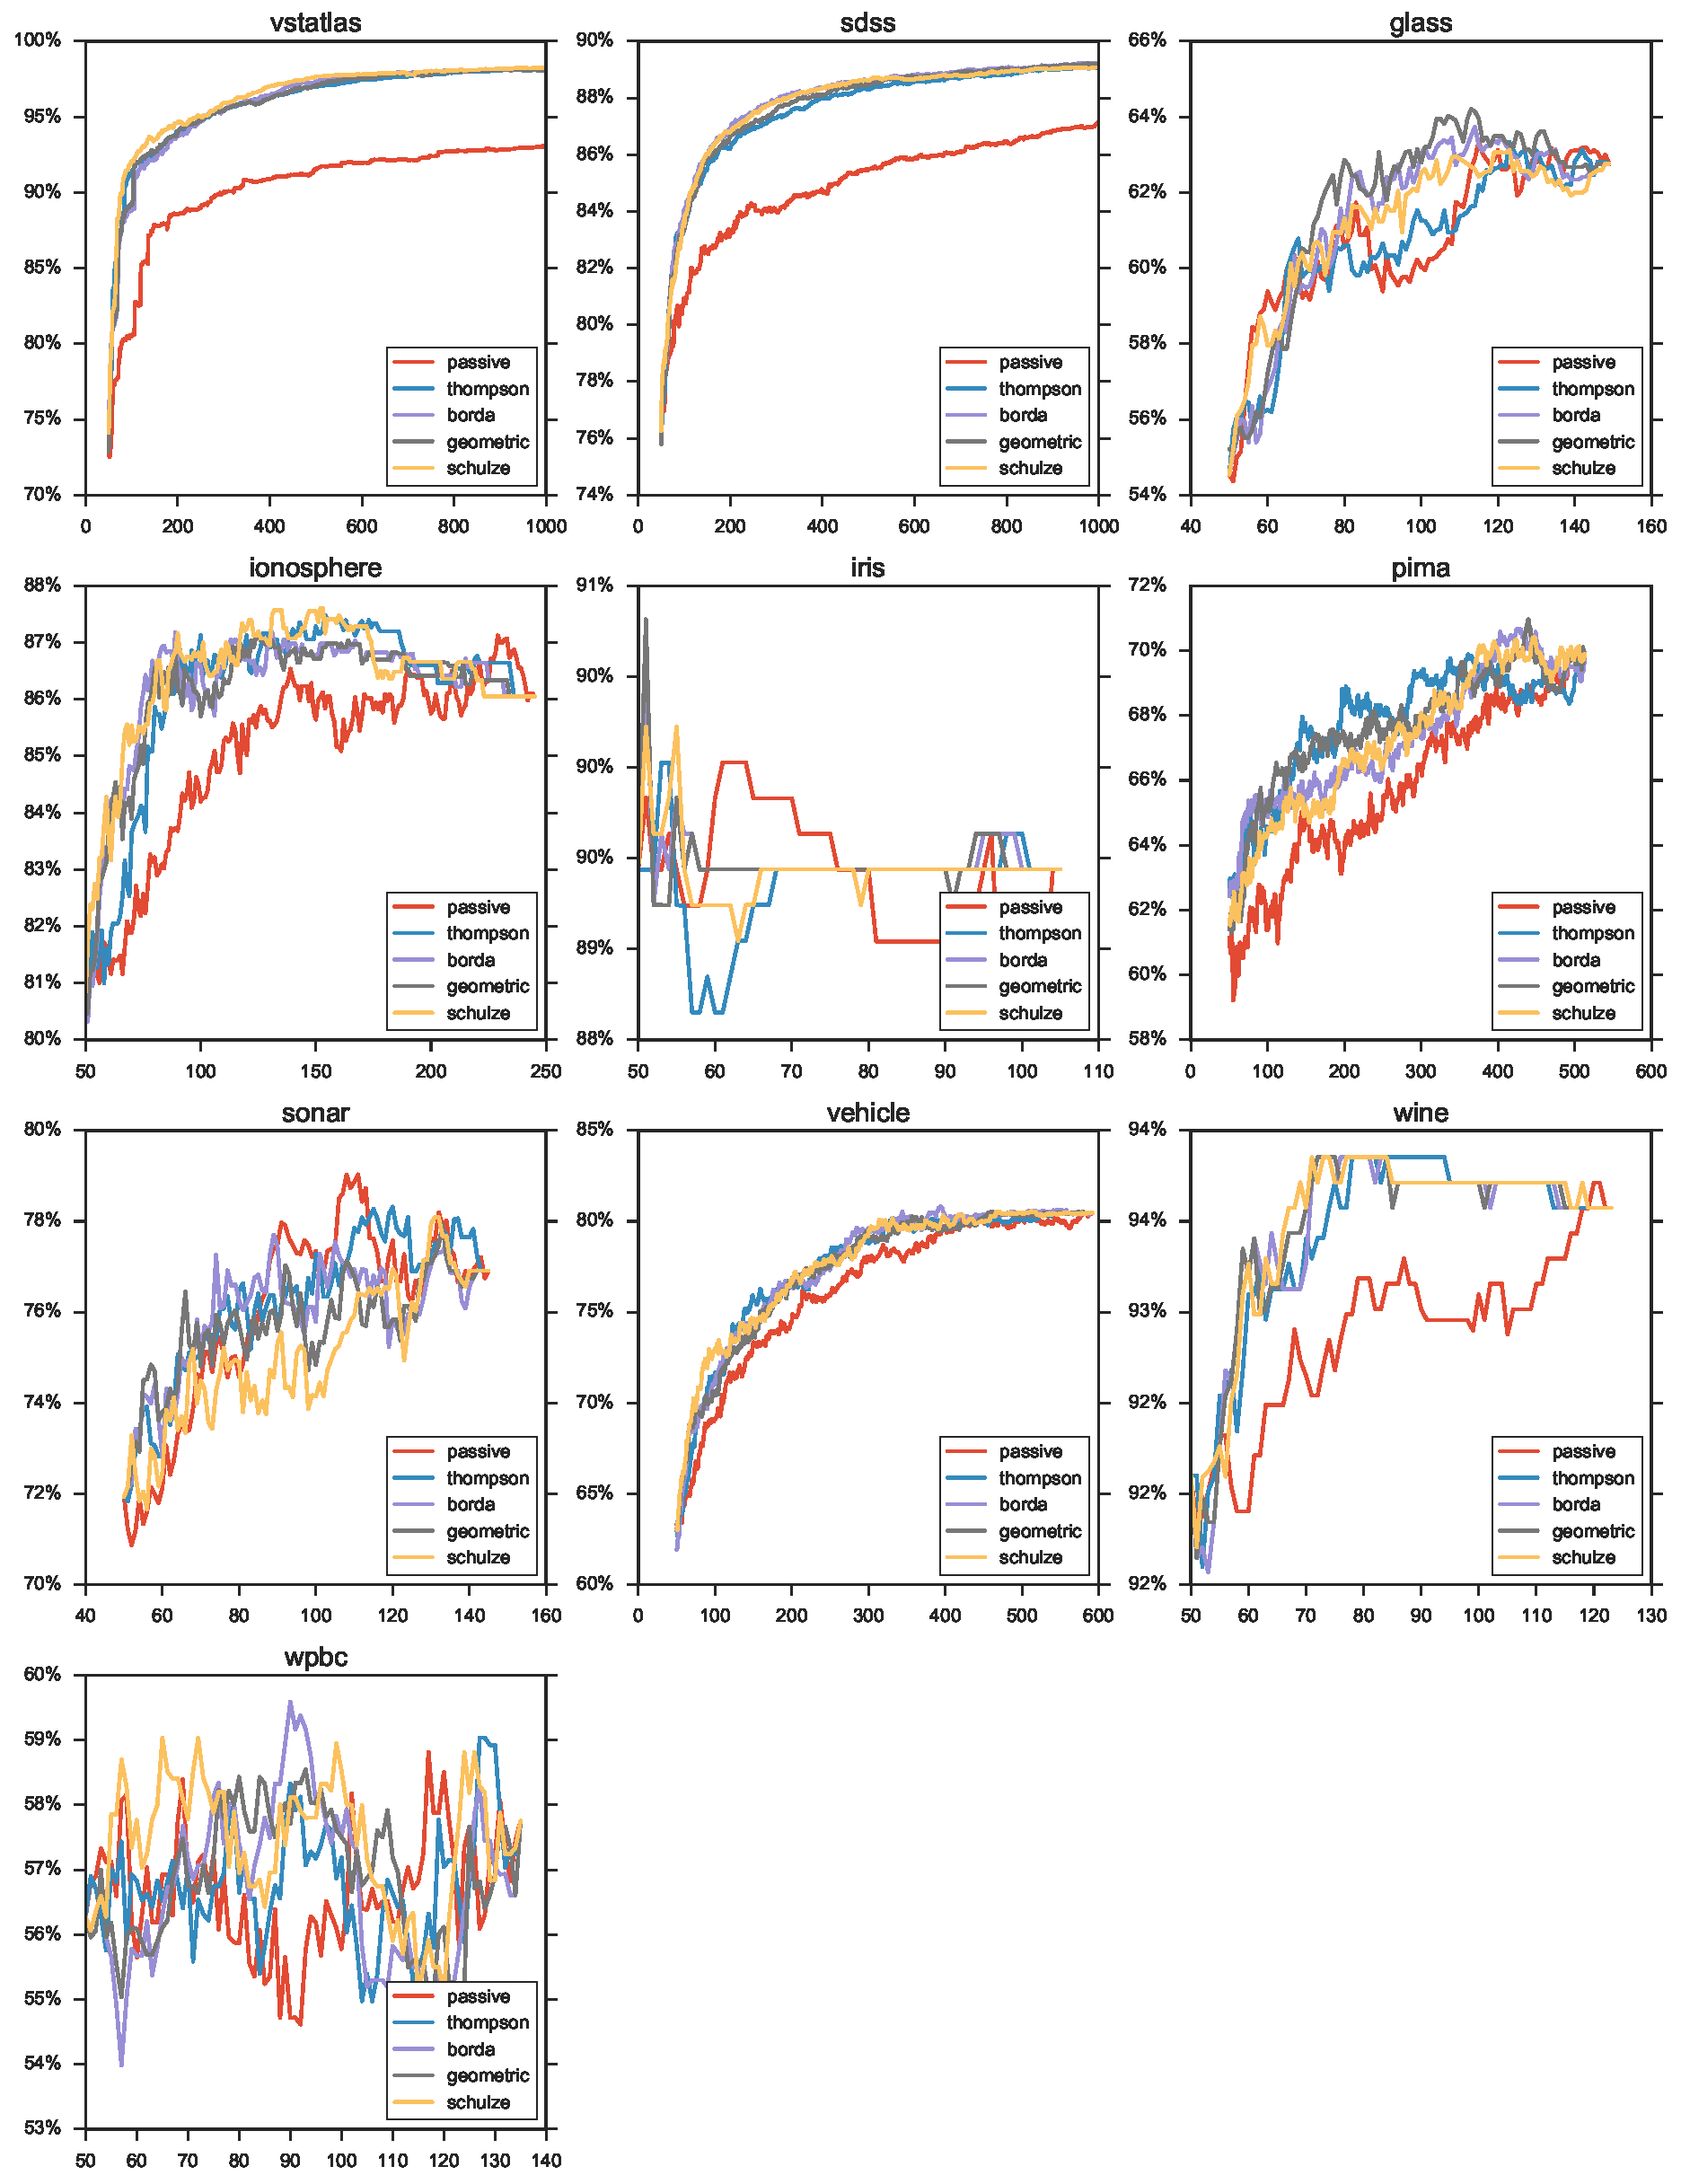
\includegraphics[width=\textwidth]{figures/learning_curves}
	\caption[Some preliminary results.]{Some preliminary results. Active learning seems
    		 to work better with bigger datasets (perhaps because the unlabelled pool
             is bigger, so it has more chance to select a good canddiate?). }
	\label{fig:learning_curves}
\end{figure}


\section*{Bits to tidy up, Appendix?}
\begin{itemize}
  \item Posterior balanced Accuracy derivation
  \item Reddening correction
  \item Feature selection, best kernel is poly degree 2
  \item Choose value of C
\end{itemize}


\section*{Acknowledgments}

So long and thanks for all the fish.

\bibliography{active}

\end{document}
